\subsection{UNet Architectures}

Introduced in \cite{ronneberger2015u-net}. U-Net is a type of convolutional neural network that's often used for biomedical image segmentation. It's named U-Net because of its U-shaped architecture.

The U-Net architecture consists of two main parts: the encoder (also known as the contracting or downsampling path) and the decoder (also known as the expanding or upsampling path).

\subsubsection{Encoder}
The encoder part of U-Net is responsible for capturing the context in the image. It works by applying repeated steps of convolution, each followed by a rectified linear unit (ReLU) and a max pooling operation. These steps help to reduce the spatial dimension of the input while increasing the depth, thereby capturing the context in the image. The output of the encoder is a set of feature maps that represent the high-level features of the input image.

\subsubsection{Decoder}
The decoder part of U-Net is responsible for localizing and segmenting the object of interest in the image. It works by applying a series of up-convolutions and concatenations with the correspondingly cropped feature map from the encoder path, followed by regular convolutions. These steps help to increase the spatial dimension and decrease the depth of the feature maps, thereby reconstructing the segmented image from the high-level features. The output of the decoder is the segmented image.

\subsubsection{Skip Connections}
The key feature of U-Net is the skip connections between the encoder and decoder. These connections allow the decoder to use information from the encoder at the same level, which helps to preserve the details and localize the object of interest in the image.

U-Net can be used for audio enhancement tasks in both the time and frequency domains. The general approach is similar in both cases: the U-Net learns to map from noisy signals to clean signals. However, the specifics of how the input and output are represented, and how the U-Net is trained, can vary depending on whether you're working in the time domain or the frequency domain.

\subsubsection{Speech Enhancement with U-Net}


In the time domain, the input to the U-Net would be a noisy audio signal, and the target would be the clean audio signal. During training, the U-Net learns to map from the noisy signal to the clean signal by minimizing a loss function that measures the difference between the U-Net's output and the clean signal. After training, you can use the U-Net to enhance new audio signals by inputting a noisy signal and getting out an enhanced signal.

% \subsubsection{Frequency Domain}
In the frequency domain, the input to the U-Net would be a spectrogram of a noisy audio signal, and the target would be the spectrogram of the clean audio signal. A spectrogram is a 2D representation of an audio signal that shows how the frequencies present in the signal change over time. During training, the U-Net learns to map from the noisy spectrogram to the clean spectrogram by minimizing a loss function that measures the difference between the U-Net's output and the clean spectrogram. After training, you can use the U-Net to enhance new audio signals by inputting a spectrogram of a noisy signal and getting out a spectrogram of an enhanced signal. The output spectrogram can then be transformed back into the time domain to get the enhanced audio signal.

\begin{figure} [h]
    \centering
    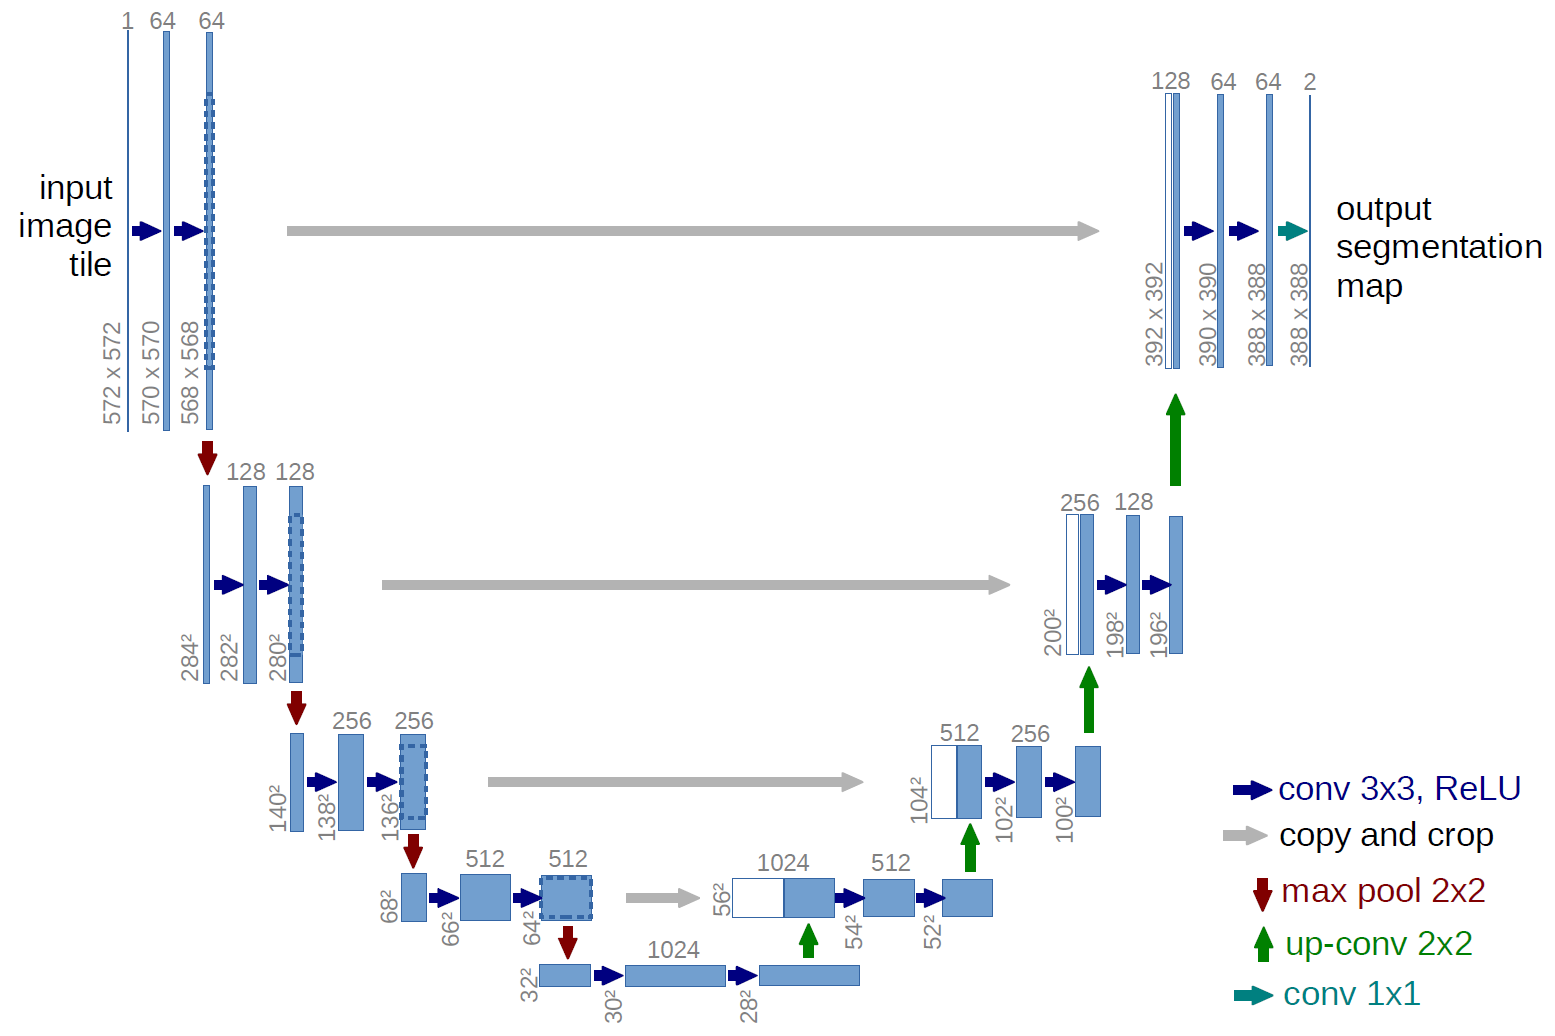
\includegraphics[width=0.75\linewidth]{images/dl/u-net-architecture.png}
    \caption{U-net architecture (example for 32x32 pixels in the lowest resolution). Each blue box corresponds to a multi-channel feature map. The number of channels is denoted on top of the box. The x-y-size is provided at the lower left edge of the box. White boxes represent copied feature maps. The arrows denote the different operations \cite{ronneberger2015u-net}.}
    \label{fig:u-net-architecture}
\end{figure}